%! TEX root = 00.tex
Fluent APIs are related to the topic of type-states.
There is a large body of research on \emph{type-states} (see
e.g., these review articles~\cite{Aldrich:Sunshine:2009,Bierhoff:Aldrich:2005})
Informally, an object that belongs to a certain type (\kk{class} in the object
oriented lingo), has type-states, if not all methods defined in this object's
class are applicable to the object in all states it may be in.

File object is the classical example: It can be in one of two states: ‟open” or
‟closed”. Invoking a \cc{read()} method on the object is only permitted when
the file is in an ‟open” state. In addition, method \cc{open()} (respectively
\cc{close()}) can only be applied if the object is in the ‟closed”
(respectively, ‟open”) state.

A recent study~\cite{Beckman:11} estimates that about~$7.2%$ of \Java
classes define protocols definable in terms of type-states.
This non-negligible prevalence raise two challenges:
\begin{enumerate}
  \item \emph{\textbf{Identification.}} Frequently, type-state receive little
    or no mention at all in the documentation. The challenge is in identifying
    the implicit type state in existing code.
        \par
    Specifically, given an implementation of a class (or more generally of a
    software framework), \emph{determine} which sequences of method calls are
    valid and which violate the type state requirement presumed by the
    implementation. \item \emph{\textbf{Maintenance and Enforcement.}} Having
    identified the type-states, the challenge is in automatically flagging out
    illegal sequence of calls that does not conform with the type-state.
        \par
    Part of this challenge is maintenance of these automatic flagging
    mechanisms as the type-state specification of the API evolves.
\end{enumerate}

\subsection{A Type State Example}

An object of type \cc{Seat}†
{%
  example inspired by earlier work of Richard Harter on the
  topic~\cite{Harter:05}.
}
is created in the \cc{down} state, but it can then be \cc{raise}d to the
\cc{up} state, and then be \cc{lower}ed to the \cc{down} state.
Such an object can be used by two kinds of users, \cc{male}s and \cc{female}s,
for two distinct purposes: \cc{urinate} and \cc{defecate}.

Thus, there are a total of six methods that might be invoked
on an instance of \cc{Seat}:
\begin{quote}
  \begin{tabular}{lll}
    \cc{male()}   & \cc{raise()} & \cc{urinate()}⏎
    \cc{female()} & \cc{lower()} & \cc{defecate()}⏎
  \end{tabular}
\end{quote}
A fluent API design specifies the order in which such calls can be made.
For example, a fluent API should recognize the sequences of
\cref{figure:toilette:legal} as being type correct.
\begin{figure}[H]
  \caption{\label{figure:toilette:legal}
  Legal sequences of calls in the toilette seat example}
  \javaInput[minipage,width=\linewidth,left=-6ex]{toilette.legal.listing}
\end{figure}

At the same time, illegal sequences as made in
\cref{figure:toilette:illegal} should be signaled as type errors.

\begin{figure}[H]
  \caption{\label{figure:toilette:illegal}
  Illegal sequences of calls in the toilette seat example}
  \javaInput[minipage,width=\linewidth,left=-6ex]{toilette.illegal.listing}
\end{figure}

To generate a fluent API that meets these requirements, one must observe that
the protocol of a \cc{Seat} is defined completely by
the DFA depicted in \cref{figure:type-state-automaton}.

\begin{figure}[H]
  \caption{\label{figure:type-state-automaton}%
    A deterministic finite automaton realizing the type states of
    class \cc{Seat}.
  }\centering
  \usetikzlibrary{automata,positioning,topaths}
\tikzstyle{state-style}=[state,draw=blue!50,very thick,fill=blue!20,node distance=13ex]
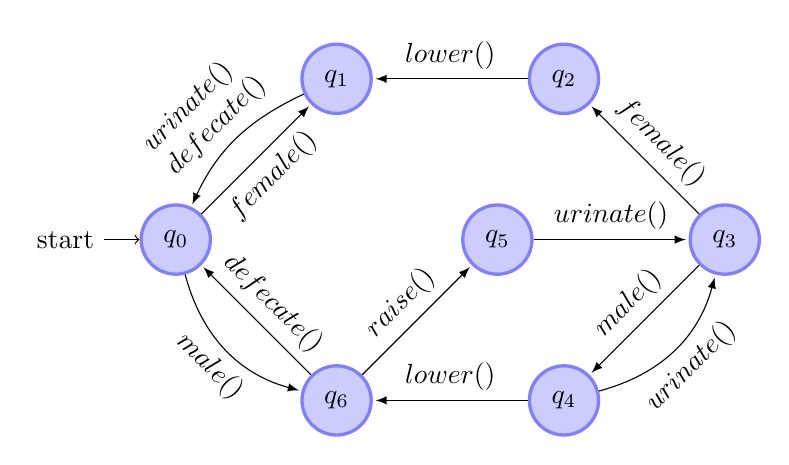
\begin{tikzpicture}
  \node[state-style,initial,initial where=above left] (q0) {$q_{0}$};
  \node[state-style] (q1) [above right= of q0] {$q_{1}$};
  \node[state-style] (q2) [right=of q1] {$q_{2}$};
  \node[state-style] (q3) [below right=of q2] {$q_{3}$};
  \node[state-style] (q4) [below left=of q3] {$q_{4}$};
  \node[state-style] (q5) [left=of q3] {$q_{5}$};
  \node[state-style] (q6) [left=of q4] {$q_{6}$};
  \path[->,above,sloped,latex-, shorten <=1pt]
  (q1) edge[below] node {$\cc{female}()$} (q0)
  (q0) edge[bend left=20,] node {\begin{minipage}{11.5ex}$\cc{urinate}()\newline \cc{defecate}()$\end{minipage}} (q1)
  (q1) edge[] node {$\cc{lower}()$} (q2)
  (q2) edge[] node {$\cc{female}()$} (q3)
  (q4) edge[] node {$\cc{male}()$} (q3)
  (q3) edge[bend left,below] node {$\cc{urinate}()$} (q4)
  (q3) edge[] node {$\cc{urinate}()$} (q5)
  (q5) edge[] node {$\cc{raise}()$} (q6)
  (q6) edge node {$\cc{lower}()$} (q4)
  (q6) edge[bend left,below] node {$\cc{male}()$} (q0)
  (q0) edge[above] node {$\cc{defecate}()$} (q6)
  ;
\end{tikzpicture}


\end{figure}

Having constructed the automaton, generating the classes and methods is
immediate by following the \emph{encoding convention}:
\begin{enumerate}
  \item A state~$q$ in the automaton is encoded as an \kk{interface}.%
        †{%
          The name of this interface is arbitrary; all that it is required is
          that names assigned to distinct states are distinct.  For readability
          sake, there is often an attempt to choose a name which makes a close
          approximation of the name of~$q$, within the limits of the language's
          syntax and Unicode vocabulary.
        }
  \item If there is an arc labeled~$ℓ$ leading from~$qᵢ$ to~$qⱼ$,
        then \kk{interface}~$qᵢ$ defines a
        method whose return type is \kk{interface}~$qⱼ$.%
        †{%
          Again, the name of this method is often selected as an approximation
          of the name of~$ℓ$.
        }
  \item The initial state~$q₀$ is made special in being the only type from
        which a fluent API call chain can start.%
        †{%
          This is achieved by generating a class~$c$ with \cc{public}
          constructor that \kk{implements} the \kk{interface} encoding
          type~$q₀$.  If no other interfaces do not have a similar~$c$, then
          clients can only start a fluent API chain by creating an instance
          of~$c$, which is
          effectively the state~$q₀$.
        }
\end{enumerate}

The result of employing these rules to our toilette example is depicted
at~\cref{figure:toilette-types}

\begin{figure}[H]
  \caption{\label{figure:toilette-types}
    A fluent API realizing the toilette seat object defined as a DFA
    in~\cref{figure:type-state-automaton}}
  \javaInput[minipage,width=\linewidth,left=-4ex]{toilette.types.listing}
\end{figure}

Using the implementation in~\cref{figure:toilette-types} we achieved
our goals regarding the legal usage examples in~\cref{figure:toilette:legal}
and the illegal usage examples in~\cref{figure:toilette:illegal}.
So far.⏎⏎

It should be clear that the type checking engine of the compiler can
be employed to distinguish between legal and illegal sequences.
